\section{Economic model}\label{sect:constraints}

As previously discussed, \shortname assumes all the parties to be rational agents. 
This section illustrates how it is possible, just by relying on that assumption, to constraint the protocol parameters in order to deploy an effective TL scheme.

Rational agents are driven by economic interests and they always try to maximize their own profit. Hence these parties have no interested in \secret itself, but only in its economic value.

Because \shortname is built upon secret sharing, it is pivotal to analyze the problem by referencing to the behavior of coalition of adversaries, and not of single users.
A coalition, \coalition, is a group of participants that team up to attack the protocol by reconstructing the secret.
To limit the attack surface, each protocol instance must then be modeled as a negative sum game to all the possible groups of adversaries. 
In other words, anyone trying to break the TL schema has to face costs greater than the maximum achievable revenues. 
To calculate the maximum revenue we focus on the best possible attack scenario, or the one in which the attacker coalition ideally completes its entire strategy, without interference by other parties.
These profit bounds are used to define inequalities among protocol parameters so that any rational agent that takes part to the protocol will comply with its rules.

In the following we address how coalitions could try to attack the protocol based on the role of its members and the time at which the attack is executed.
For the sake of clarity, Subsections~\ref{sect:mal_sha} and ~\ref{sect:mal_own} does not take into account the \texttt{\algowhistleblowshare} function, which will be discussed in as a general case in Subsection~\ref{sect:impact_wh}.


%In the description we gave so far only the basic protocol operating scheme was presented, but no mention was made about the ratio between the economic constraints that have to be imposed on the parameters.
% The protocol is in fact vulnerable because it is exposed to coalitions of attackers that can be both {\em internal} and {\em external} to the TL mechanism.
%However, since the economic (dis-)incentives are the only way to achieve the compliance of rules, it is required to identify the targets which these rules are addressed to, so that the desired outcome is obtained. In particular, the target of the described protocol is strictly time dependent, as the participants have to protect the secrecy of \secret before the disclosure time, and as after \td they have to make sure it to be disclosed.

\begin{algorithm}[t]
	\caption{SC function to disclose the share after \td}\label{algo:disclose}
	\begin{algorithmic}[1]
		\MyAlgBlock{input}
		\Desc{$sc$}{\hspace*{1.5em}smart contract identifier}
		\Desc{$i$}{\hspace*{1.5em}index of the submitted share}
		\Desc{$\share_i$}{\hspace*{1.5em}the $i$-th share}
		\vspace{0.6em}
		\Procedure{Disclose}{$sc, i, \share_{i}$}
		\If{$sc.\state = \statelocked$ \textbf{and} $sc.\states[i] = \statepaid$}
		\If{$\primtime \geq sc.\td$ \textbf{and} $\primtime < sc.\te$}
		\If {$\primhash{\share_i} = sc.\Cshare{}[i]$}
		\State $sc.\shares \left[ i \right] \gets \share_{i}$
		\State $sc.\numdisclosed\ += 1$
		\State $sc.\states[i]\gets \statedisclosed$
		\State $p_1 \gets sc.\numdisclosed \ge sc.\K$
		\State $p_2 \gets \primtime > \te$
		\State $p \gets p_1 \wedge p_2$
		\State $\primwithdraw{sc}{caller}{\RH}{p}$
		\EndIf
		\EndIf
		\EndIf
		\EndProcedure
	\end{algorithmic}
\end{algorithm}

\subsection{Protection against malicious shareholders}\label{sect:mal_sha}

Being the shareholder rational agents, they will consider if is worth to try breaking the TL before \td or not.
To perform a successful attack, a shareholder has to team up with other $\K - 1$ ones in order to reconstruct \secret, sell it to a buyer, and whistleblow it\footnote{\ The coalition \coalition could setup an additional contract between \coalition and the buyer to be sure to gain both \V and \Wsecret.}.
In that event, \coalition would earn at most by selling and by whistleblowing, leading the protocol to failure. 
The alternative, i.e. do not break the TL and submit the $k$ shares after \td, would lead to a gain equal to the sum of the rewards. 
To avoid the first scenario we can impose:
%
%\begin{equation}\label{eqbalance1}
%\tag{$1^*$}
$\K \cdot \RH  > \V + \Wsecret$.
%\end{equation}

Yet, in order to to earn $\K \cdot \RH$, the coalition \coalition should wait until \td, whereas $\V + \Wsecret$ could be collected earlier.
For this reason, in \shortname we use a stricter formulation of the constraint, obtained by comparing the revenue earned by whistleblowing and the total amount of bids already paid \coalition to get the shares:

\begin{equation}\label{eqcoscom2}
\K \cdot \BH > \V + \Wsecret
\end{equation}


The first constraint addresses secrecy (time $t < \td$), however, when the disclosure time passes, the objective of the TL turns into facilitating the disclosure.
In this setting, threshold cryptography may obstacle the release of \secret, offering additional opportunities to malicious shareholders and coalitions of them.
In fact, $\N - \K + 1$ shareholders could wait for $\K - 1$ others to submit their share and then lead the TL instance to a stall by refusing to submit their ones and wait for a buyer willing to pay \V to gain access to the secret.
To avoid this issue, we introduce the constraint:  

\begin{equation}\label{eqcoscom4}
(\N - \K + 1) \cdot \RH  > \V
\end{equation}

Here the contribution of the term $\Wsecret$ disappears as the role of whistleblower is no longer admissible after \td. The inequality holds because the shareholders are authorized to collect their rewards \RH only in case the TL results in a successful outcome\footnote{An alternative approach to reduce stalls without the need of a termination time and deferred rewards would be to grant an extra reward \extrareward to the first \K shareholders that submit the share after \td.
%Timely payment of rewards would encourage this type of attack, as in some situations \coalition could use it to reduce the entry fee while still not publicly disclose the secret (i.e., not write it to the smart contract).
%Such a bonus --- which in total amounts to $\K \cdot \extrareward$ --- would be paid from \PO.
%The latter would contribute positively to inequalities~\ref{eqbalance1} and ~\ref{eqcoscom2}.
%anyhow foreseeing race conditions is not strictly compulsory.
}
(i.e., at least \K shares are submitted before the termination time \te).


\subsection{Protection against malicious owners}\label{sect:mal_own}

All the considerations made about the rationality of the shareholders must also be applied to the owner.
As \owner knows the secret in advance, she could setup fake TL instances for the sole purpose of invoking the \texttt{\algowhistleblowsecret} function and obtain \Wsecret, if this would end up having a positive economic return.
%
%Anyone in possession of the secret can act as a whistleblower, then the owner could be interested in setting up a fake protocol to get $\Wbonus_{\secret}$.
To enforce a negative outcome for this scenario, we need to add the following constraint:

\begin{equation}\label{eqbalance3}
\PO > \Wsecret
\end{equation}

%Since the penalties are enforced by smart contracts, someone might be tempted to prevent the owner from executing the whistleblow protocol, thus replacing~\ref{eqbalance3} by an identity check.  Yet, there is no way to forbid the owner from teaming up with a shareholder, and forming an malicious mixed coalition.  Such a case should be addressed by the addition of:

%\begin{equation}\label{eqbalance7}
%\PO + \BH > \Wbonus_{\secret}
%\end{equation}

%which is a less stringent constraint than~\ref{eqbalance3}.


\subsection{Impact of share whistleblowing function}\label{sect:impact_wh}

The ability to whistleblow shares, needed to prevent selling shares, opens up to more complex strategies that can be performed by a coalition.
A coalition \coalition composed by \K shareholders could in fact submit some of the controlled shares to the smart contract before whistleblowing the secret, in order to maximize the revenue.

As the coalition is composed by rational agents, it is possible to determine the optimal number \jopt of shares that the coalition could submit before incurring into penalties or advantaging other participants.
%Indeed, submitting $k$ shares before \td leads to the TL failure, and therefore the impossibility of earning $\Wbonus_{\secret}$, which we remind is greater than $\Wbonus_{\share}$. 
Whistleblowing a share is in fact a public event, observable by all the participants, so it could itself trigger other participants' strategies.
%Another aspect we point out is that a share whistleblow is an event observable by all the participants, as the state smart contract is publicly readable. 

The values \N and \K, the number of total shareholders and the threshold, identify two distinct cases to compute  \jopt.
\begin{enumerate}
	\item {\em Case $\K > \lfloor \N/2 \rfloor $ }\\
	A \K-shareholders coalition \coalition is the only one able to break the TL; $\jopt = 2\K-\N-1$ shares can be submitted while still preventing the other $\N-\K$ shareholders to reconstruct \secret. 
	The extra-revenue is then:
	$$ \Wer = \left( 2\K - \N - 1 \right) \cdot \Wshare$$
	\item {\em Case $ \K \le \lfloor \N/2 \rfloor $}\\
	A \K-shareholders coalition $\coalition^\prime$ is not the only one able to break the TL. 
	Each time a share is whistleblown, all the other $\N-\K$ shareholders and their possible coalitions are triggered as a side effect.
	%Let's assume that a first coalition $\coalition ^\prime $ whistleblows a share;
	%$\coalition ^\prime $ would earn $\Wshare$, while losing the bid \BH paid to obtain the share.
	%
	%, accordingly a second coalition $\coalition ^{\prime \prime} $ might form.
	%, $\coalition ^{\prime \prime} $ would save \BH in case of an hypothetical \secret reconstruction.
	%As $\BH > \Wbonus_{\share}$, then $\coalition ^{\prime \prime} $ would become the most dangerous attacker. \\
	%A second coalition $\coalition ^{\prime \prime}$ that only consists of $\K-1$ shareholders would now be able to reconstruct the secret. 
	Thus, every time a share is whistleblown, the threshold \K is weakened. 
	In general, when $i$ shares have been whistleblown, a coalition $\coalition^i$ formed by $\K-i$ shareholders would gain the ability to reconstruct the secret \secret. $\coalition^i$ having paid only $(\K-i) \cdot \BH$ to get its shares. 
	For this reason, the initial coalition \coalition formed by \K shareholders needs to determine the optimal number of shares \jopt to be whistleblown so that there is no other coalition that can profit from the weakening of \K. In particular, \coalition can determine \jopt by solving the following:
	$$\jopt = \operatorname*{max}_i\ \{i | (\K-i) \cdot \BH > \V + \Wsecret,\ i \in 1,\ldots,\K-1 \}$$
	%, while benefit from a cost saving of $i \cdot \BH$ while performing the attack. So, if $i_{inv}$ so that
	%$$
	%\begin{cases}
	%\left( \K - i_{inv} \right) \cdot \BH < \V + \Wbonus_{\secret} \\
	%\left( \K - i_{inv} + 1 \right) \cdot \BH > \V + \Wbonus_{\secret} 
	%\end{cases}
	%$$
	If such a \jopt exists, by keeping the assumption of rational agents, the coalition \coalition can submit \jopt shares while still being sure that no other smaller coalition will whistleblow the secret.
	The extra-revenue is then:
	%$$ \bigtriangleup W_{er} = \left( i_{inv} - 1 \right) \cdot \BH$$
	$$ \Wer = \jopt \cdot \Wshare$$
	 
\end{enumerate} 

We can factor the two cases and formulate a stricter version of Equation~(\ref{eqcoscom2}) that takes into account the possible extra revenue by constraining:

%\begin{equation}\label{eqbalance1w}
%\K \cdot \RH  > \V + \Wbonus_{\secret} + \bigtriangleup W_{er}
%\end{equation}

\begin{equation}\label{eqcoscom2w}
\K \cdot \BH > \V + \Wsecret + \Wer
\end{equation}



%\subsection{Variations}\label{sect:variat}

%In this subsection we show how the proposed model can be easily extended to achieve additional goals.

%\subsubsection{Resiliency}
%Until now we always assumed all the parties to be perfect rational agents. However, a number of shareholders \lost might expose their share (i.e., because of negligence, external attacks). In such a case, a coalition of $\K - \lost$ malicious shareholders could reconstruct the secret without the need of sharing the reward with the shareholders that lost their shares.
%To prevent this possibility, the owner could define \lost to be the upper bound of the number of shares that can go misplaced. By integrating this information into equation~(\ref{eqcoscom2}), we are able to nullify the gain for such a coalition:
%\begin{equation}\label{eqcoscom3}
%(\K - \lost) \cdot \BH  > \V + \Wbonus
%\end{equation}




%\paragraph*{Reducing owner pawn}



%pursuing the will to play against the system (i.e., against the shareholders), or could misbehave because of giving up to keep interest into \secret and then trying to get the whistleblower bonus.
%
%To dis-incentivize his misbehavior, we include in our model a reward \RO that the owner will receive in case of successful executions of the protocol.
%
%To foresee a reward to $\owner$ could at first sight look strange in the design of a TL primitive, but as we consider him to be alive at disclosure time~\footnote{The scenario which we imagine our TL protocol to be suitable to is different from the traditional one, more specifically we do not focus on very long time distances. We remind the reader to discussion section for further details.} basically need to avoid the owner to game the system. \todo{Meglio specificare bene prima lo scenario di interesse o dopo?}

%By defining a relation between \Wbonus and \RO we can impose that even if the owner loses interest in keeping \secret private, he will have a greater benefit from a successful execution of the protocol compared to whistleblowing the secret:

%The introduction of \RO requires to adapt the equality~(\ref{eqbalance}), since this reward has to be paid by the owner:

%\begin{equation}\label{eqbalance4}
%\PO = \N \cdot \profit  + \RO
%\end{equation}

%This way we enforce that the costs for the owner are always greater than the benefits he can obtain from the system (effectively dis-incentivizing his misbehavior). In fact, by combining Equation~(\ref{eqbalance3}) and Equation~(\ref{eqbalance4}), we can derive:

%\begin{equation}\label{eqbalance5}
%\PO > \RO > \Wbonus
%\end{equation}


%\subsubsection{Avoiding owner reward}

%Foreseeing a reward \RO for the owner after \td might be considered as an active role for the owner after \td. This is acceptable in scenarios in which the owner wants to safeguard the publication of the secret \secret at time \td, even though she is expected to return online at a later time to claim her reward.

%As described in Section~\ref{sect:protection}, the owner reward \RO is necessary to prevent gains from an owner who is willing to setup a fake protocol just to claim the whistleblower bonus \Wbonus (at the expenses of the shareholders). 
%An alternative to avoid the owner reward \RO, would be to limit the attack surface of a malicious owner. This can be done by limiting the role of the whistleblower only to the shareholders \shareholder (i.e., the owner can not claim the whistleblower bonus). This is not enough as an attacker could take part to the \shortname protocol with two identities, one in which he plays as the owner, and one in which he plays as a shareholder. To prevent any economic gain from this practice, we can introduce the following additional constraint.

%\begin{equation}\label{noro}
%\PO + \BH > \Wbonus
%\end{equation}

%This way, any coalition of the owner, who knows \secret, and a shareholder, needed to whistleblow, would imply a negative gain.

%\begin{comment}
%UNCOMMENT THIS WHEN FINAL.

%\begin{figure}[tp]
%	\centering
%	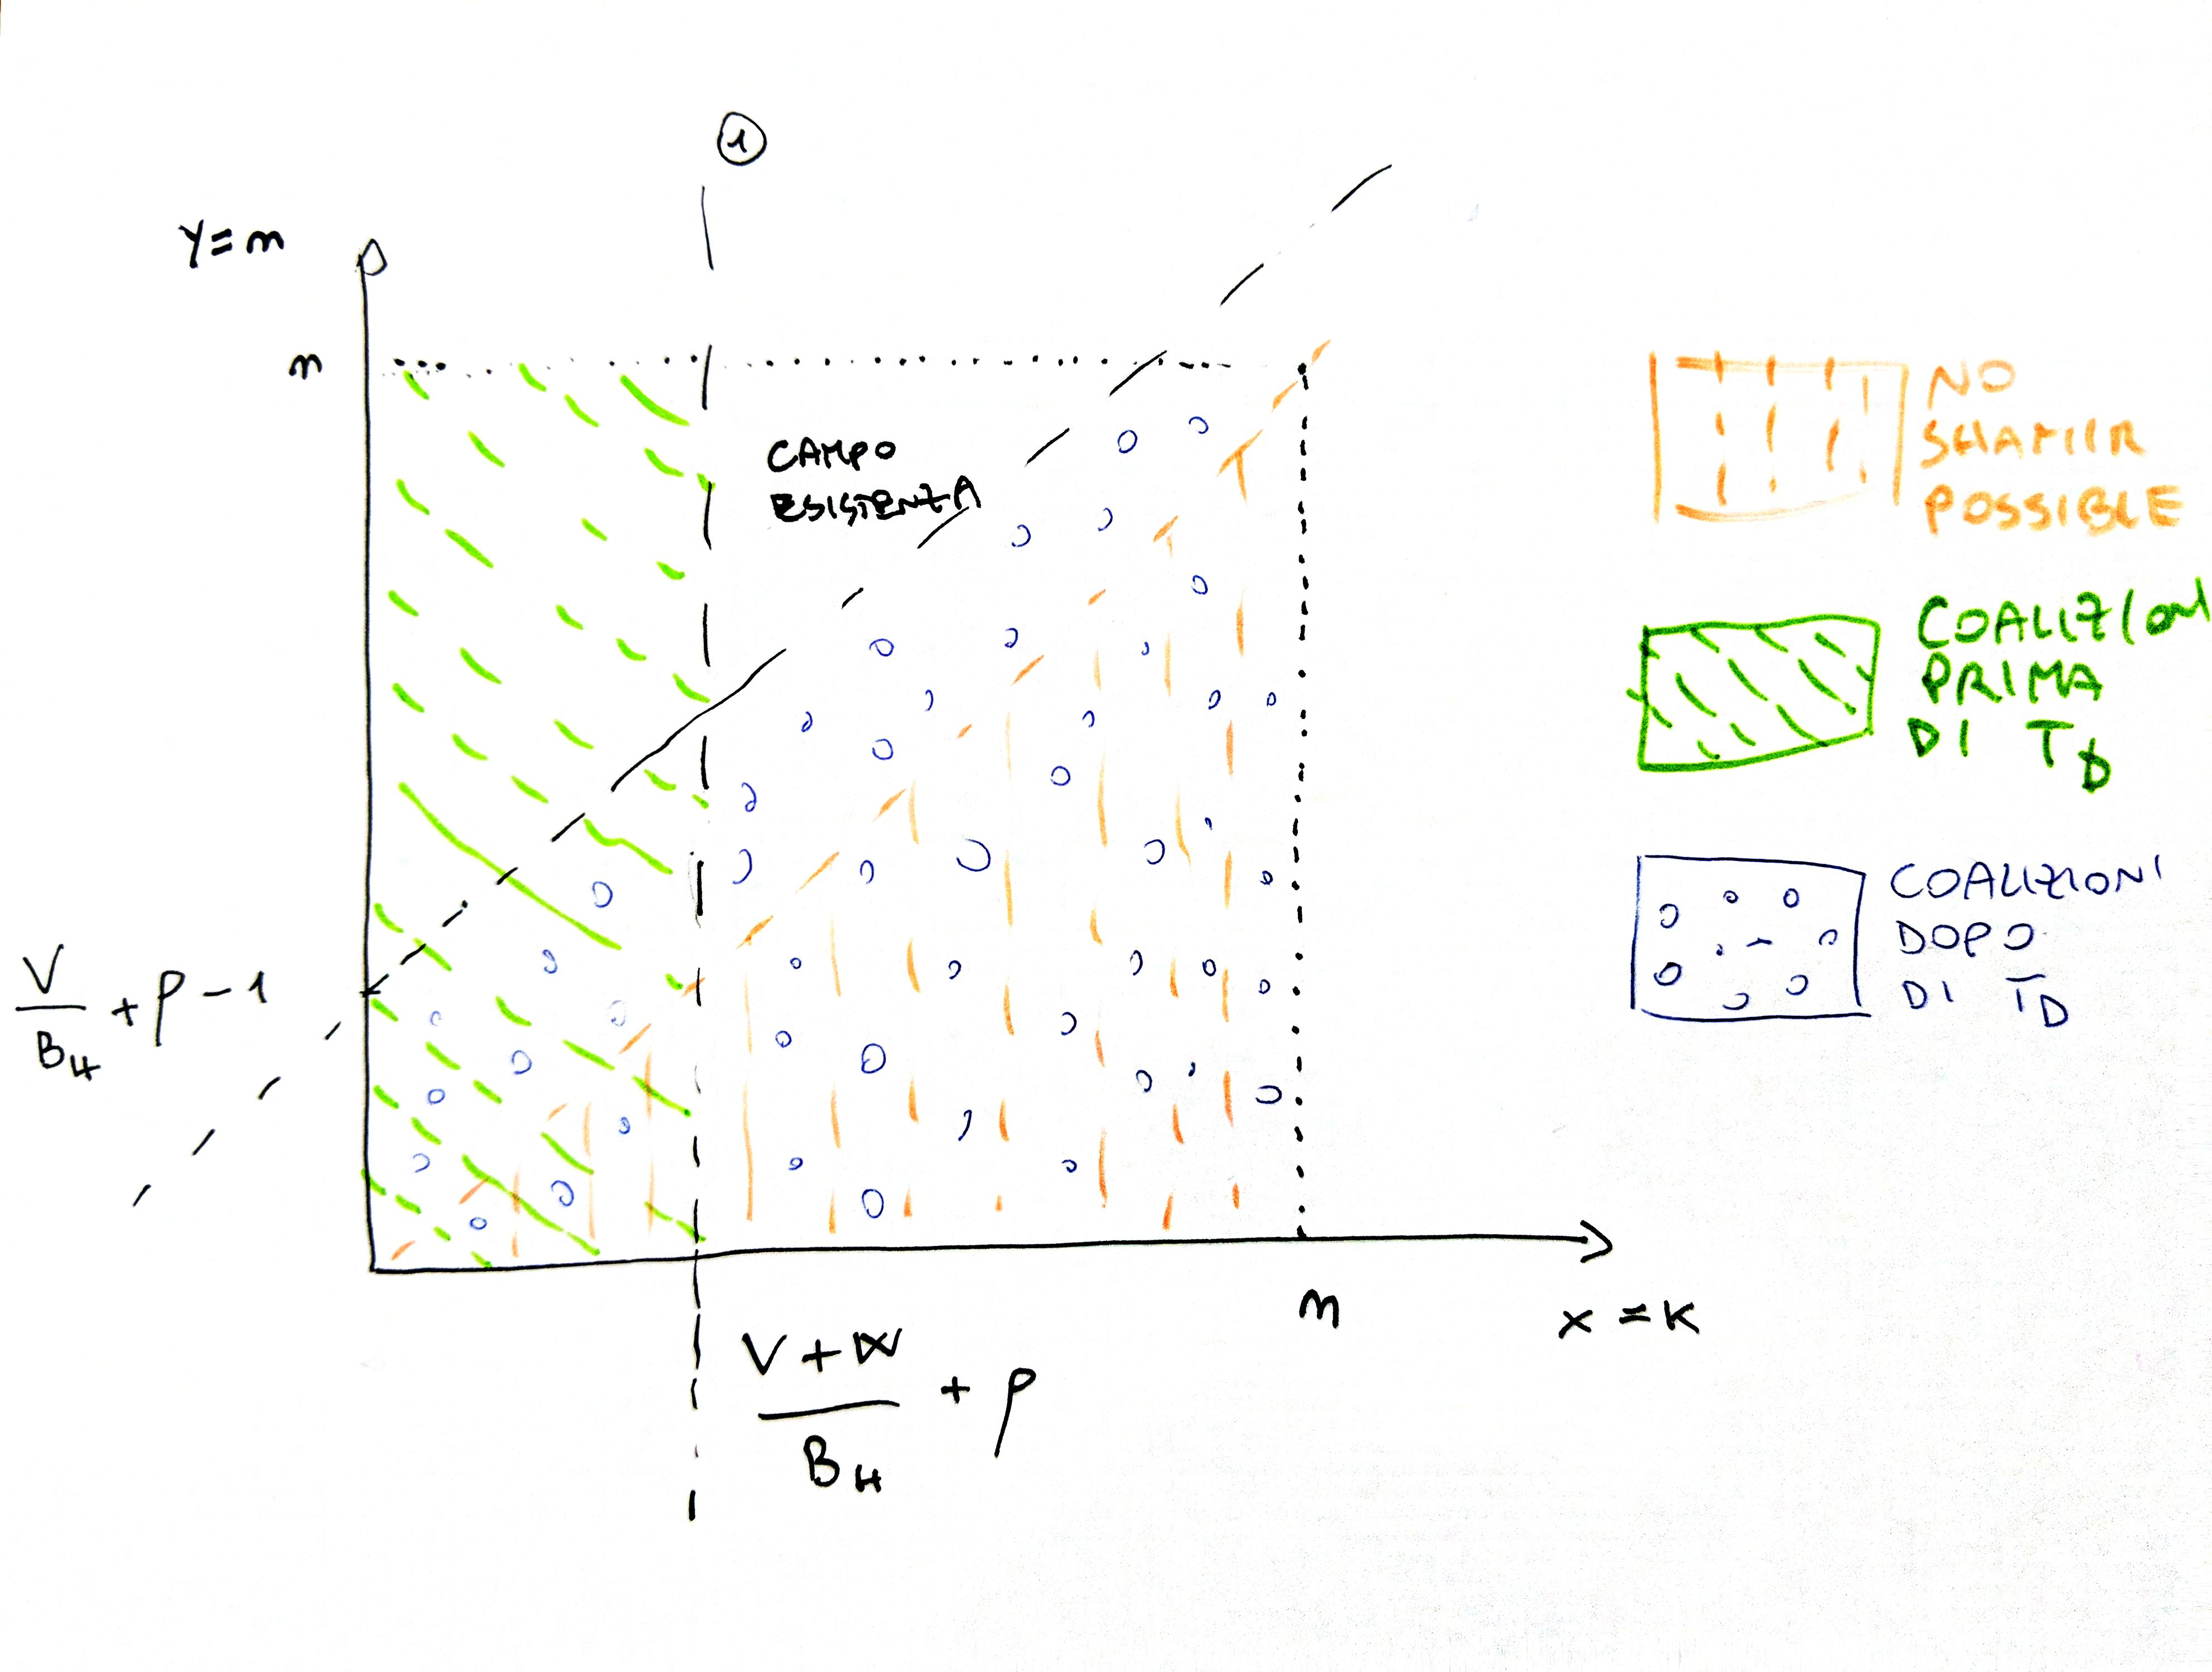
\includegraphics[width=\columnwidth]{constraints}
%	\caption{{\em \shortname} constraints.}
%	\label{fig:constraints}
%\end{figure}
%
%due righe per introdurre la rappresentazione grafica dei vincoli e del campo di esistenza del modello, ATTENZIONE TOGLIERE DALLA FIGURA IL CONTRIBUTO DELLE VARIAZIONI
%\end{comment}